\section{El teorema de Gram-Schmidt}
Dado un espacio de Hilbert $V$
y $W$ un subespacio de dimensión finita de $V$,
en ocasiones nos interesará contar no sólo con una
base de Hamel $W$, sino con una base ortonormal de este
(recuerde que, en el caso finito dimensional, toda
BON es una base Hamel).
 
El siguiente resultado nos permite lograr justamente eso;
la esencia del teorema de Gram-Schmidt es el reemplazar una base
$S=\{ v_{0}, \ldots ,v_{n-1} \}$ de un subespacio 
$W := span(S)$ de dimensión finita de $V$ 
por una base ortogonal $S'$ para este, que
fácilmente puede normalizarse multiplicando a cada elemento 
de $S'$ por el reciproco de su norma.
Al proceso descrito a continuación lo llamaremos
el \textbf{proceso de ortonormalización de Gram-Schmidt.}
y lo abreviaremos como ``G-S''.\\

\begin{teo} \label{Teo:Gram-Schmidt}
(\textbf{de Gram-Schmidt}, \cite{friedberg} p.344): 
Sean $V$ un espacio vectorial
con producto punto, $S=\{ v_{k} : \hspace{0.2cm} 0 \leq k \leq n-1 \}$ un
subconjunto linealmente independiente de $V$. 
Sean los vectores

\[
\begin{split}
\xi_{0}:= & v_{0}, \\
\xi_{k} := & v_{k} - \suma{j=0}{k-1}{
\frac{\langle v_{k} , \xi_{j} \rangle}{
\langle \xi_{j} , \xi_{j} \rangle}  \xi_{j}},
\hspace{0.2cm} k=1, \ldots ,n-1.
\end{split}
\]
\noindent
El subconjunto 
$S':=\{ \xi_{k} : \hspace{0.2cm} 0 \leq k \leq n-1  \}$ de $V$
es ortogonal y genera el 
el mismo espacio que $S$.
\end{teo}


La ventaja de la formulación del teorema
de Gram-Schmidt dada en \ref{Teo:Gram-Schmidt}
es que esta
da explícitamente la forma de calcular a los
elementos de la base ortogonal para el subespacio
finito-dimensional, pero,
para nuestros fines, una formulación que
involucre proyecciones ortogonales sobre espacios
será preferible. De este modo la geometría
que hay detrás del proceso puede
vislumbrase mejor. 


\begin{prop} \label{Prop:Gram-Schmidt2}
\textbf{(versión del teorema de Gram-Scmidt en términos de
proyecciones)}
Sean $V$ un espacio vectorial con producto punto,
\[
S=\{ v_{k} : \hspace{0.2cm} 0 \leq k \leq n-1 \}
\] un subconjunto
linealmente independiente de $V$ y
\[
S' =\{ \xi_{k} : \hspace{0.2cm} 0 \leq k \leq n-1 \}
\] el subconjunto
ortogonal que resulta de aplicar el proceso de
Gram-Schmidt \ref{Teo:Gram-Schmidt} a $S$. \\

Si para cada $0 \leq k \leq n-1$ se define al subespacio
\[
W_{k}= span(v_{0}, \ldots , v_{k}) 
\]
de $V$, entonces, para toda $1 \leq k \leq n-1$
se tiene que 
\begin{center}
\framebox{ $\xi_{k}=v_{k}- \Pi_{W_{k-1}}(v_{k})$.}
\end{center}
\end{prop}
\noindent
\textbf{Demostración.}

\begin{marginfigure}
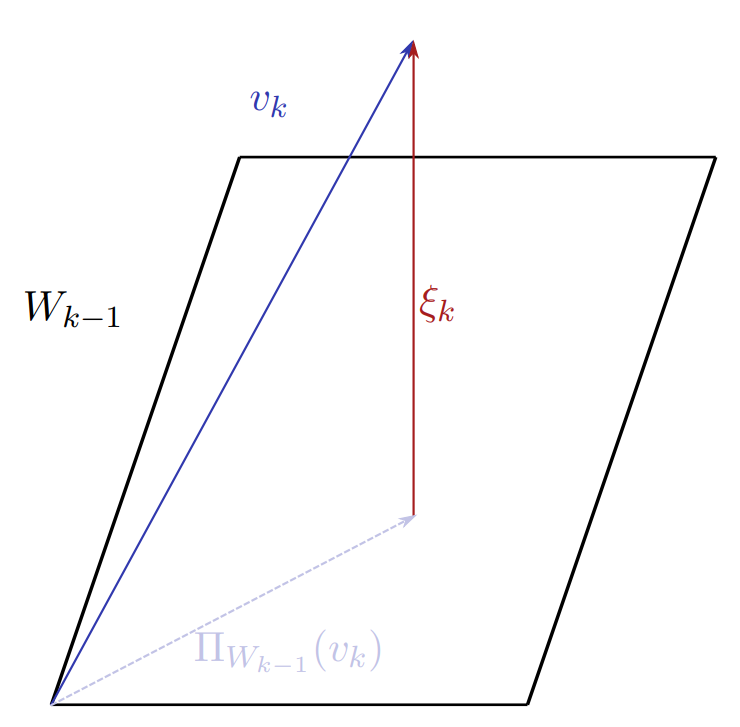
\includegraphics[scale=0.25]{GS_fig} 
		\caption{Ilustrando el proceso de Gram-Schmidt formulado 
		en términos de proyecciones.}
\end{marginfigure}

\noindent
Sea $1 \leq k \leq n-1$.
Según el teorema de Gram-Schmidt (\ref{Teo:Gram-Schmidt}),
\begin{equation}
\label{eq10: 11ap}
W_{k-1}=span(\xi_{0}, \ldots , \xi_{k-1}).
\end{equation}


Si mostramos que
\begin{itemize}
	\item el vector $v_{k}-\xi_{k}$ es elemento
	del espacio $W_{k-1}$, y que
	\item $\xi_{k}=v_{k}-(v_{k}-\xi_{k})$
	es elemento de $W_{k-1}^{\perp}$,
\end{itemize}
por la unicidad establecida en
el teorema de la proyección ortogonal \ref{Teo:proyOrt}
podremos concluir la igualdad deseada. \\
Lo primero es claro, pues, según las fórmulas
dadas en el teorema \ref{Teo:Gram-Schmidt},
\[
v_{k}-\xi_{k}= 
\suma{j=0}{k-1}{
\left( \frac{v_{k} \cdot \xi_{j}}{\xi_{j} \cdot \xi_{j}} \right) \xi_{j}} \in W_{k-1}.
\]
Lo segundo se sigue de observar que
$\xi_{k}$ es ortogonal a los vectores $\xi_{0}, \ldots , \xi_{k-1}$;
como estos conforman una base para $W_{k-1}$
(c.f. \eqref{eq10: 11ap}), concluimos
que $\xi_{k} \in W_{k-1}^{\perp}$.

%\begin{figure}[ht]
%   \centering
%   \incfig{ConFab}
% \end{figure}

\QEDB
\vspace{0.2cm}